\documentclass[11pt]{article}
\usepackage{amsmath, amssymb, amsthm, graphicx, enumerate}
\usepackage[margin=1in]{geometry}

\title{Parallelzing an All-Pairs Shortest Path Algorithm}

\author{Bangrui Chen (bc496), Markus Salasoo (ms933), and Calvin Wylie (cjw278)}

\begin{document}

\maketitle

\section*{Introduction}

\section*{MPI Implementation}

We implemented a parallel version of the shortest path algorithm using the
Message Passing Interface (MPI).
In our implementation, each processor is responsible for updating a portion of 
the shortest path matrix $l$.  Specifically, we partition by column, so that 
the processor labelled $k$ (for $k = 1, \ldots, p$), updates $l_{ij}$ for 
$j \in J_k$, where the $(J_k)_{1 \leq k \leq p}$ define a partion of 
$\{1, 2, \ldots, n\}$.
With this strategy the computation pattern for updating the shortest path matrix
remains the same, we are simply looping over a smaller sets of columns.

After each processor has finished updating it's corresponding columns in
the update $l_{ij}^{s+1} = \min_k \{ l^s_{ik} + l^s_{jk} \}$, we call
\emph{MPI\_Allgather} so that each processor gets the fully updated $l^{s+1}$
for the next step.  Each processor also keeps a local ``done'' flag that will
be true if nothing was updated.  In order to determine whether to terminate
or not, we call \emph{MPI\_Allreduce} with a logical AND operator on the local
done flags.

\subsection*{Strong Scaling}

\subsection*{Weak Scaling}

\section*{Scaling Study}
We did both strong scaling and weak scaling study using the openmp code.
\subsection{Strong Scaling}
In the strong scaling, we compare parallel to serial time for a fixed size problem. Since the graph is randomly generated, for each experiment, we did 10 simulation and use the average time as their running time. Here we choose the problem size $n=2000$ and the speedup is summarized in left plot of Figure~\ref{scaling}. As can be seen from the left plot of Figure~\ref{scaling}, when we increase the number of threads from 1 to 12, the speed up grows linearly with respect to the number of threads. After 12 threads, the speedup doesn't grow linearly due to the excess amount of overheading and synchronization.

\begin{figure}
\caption{scaling study}
\label{scaling}
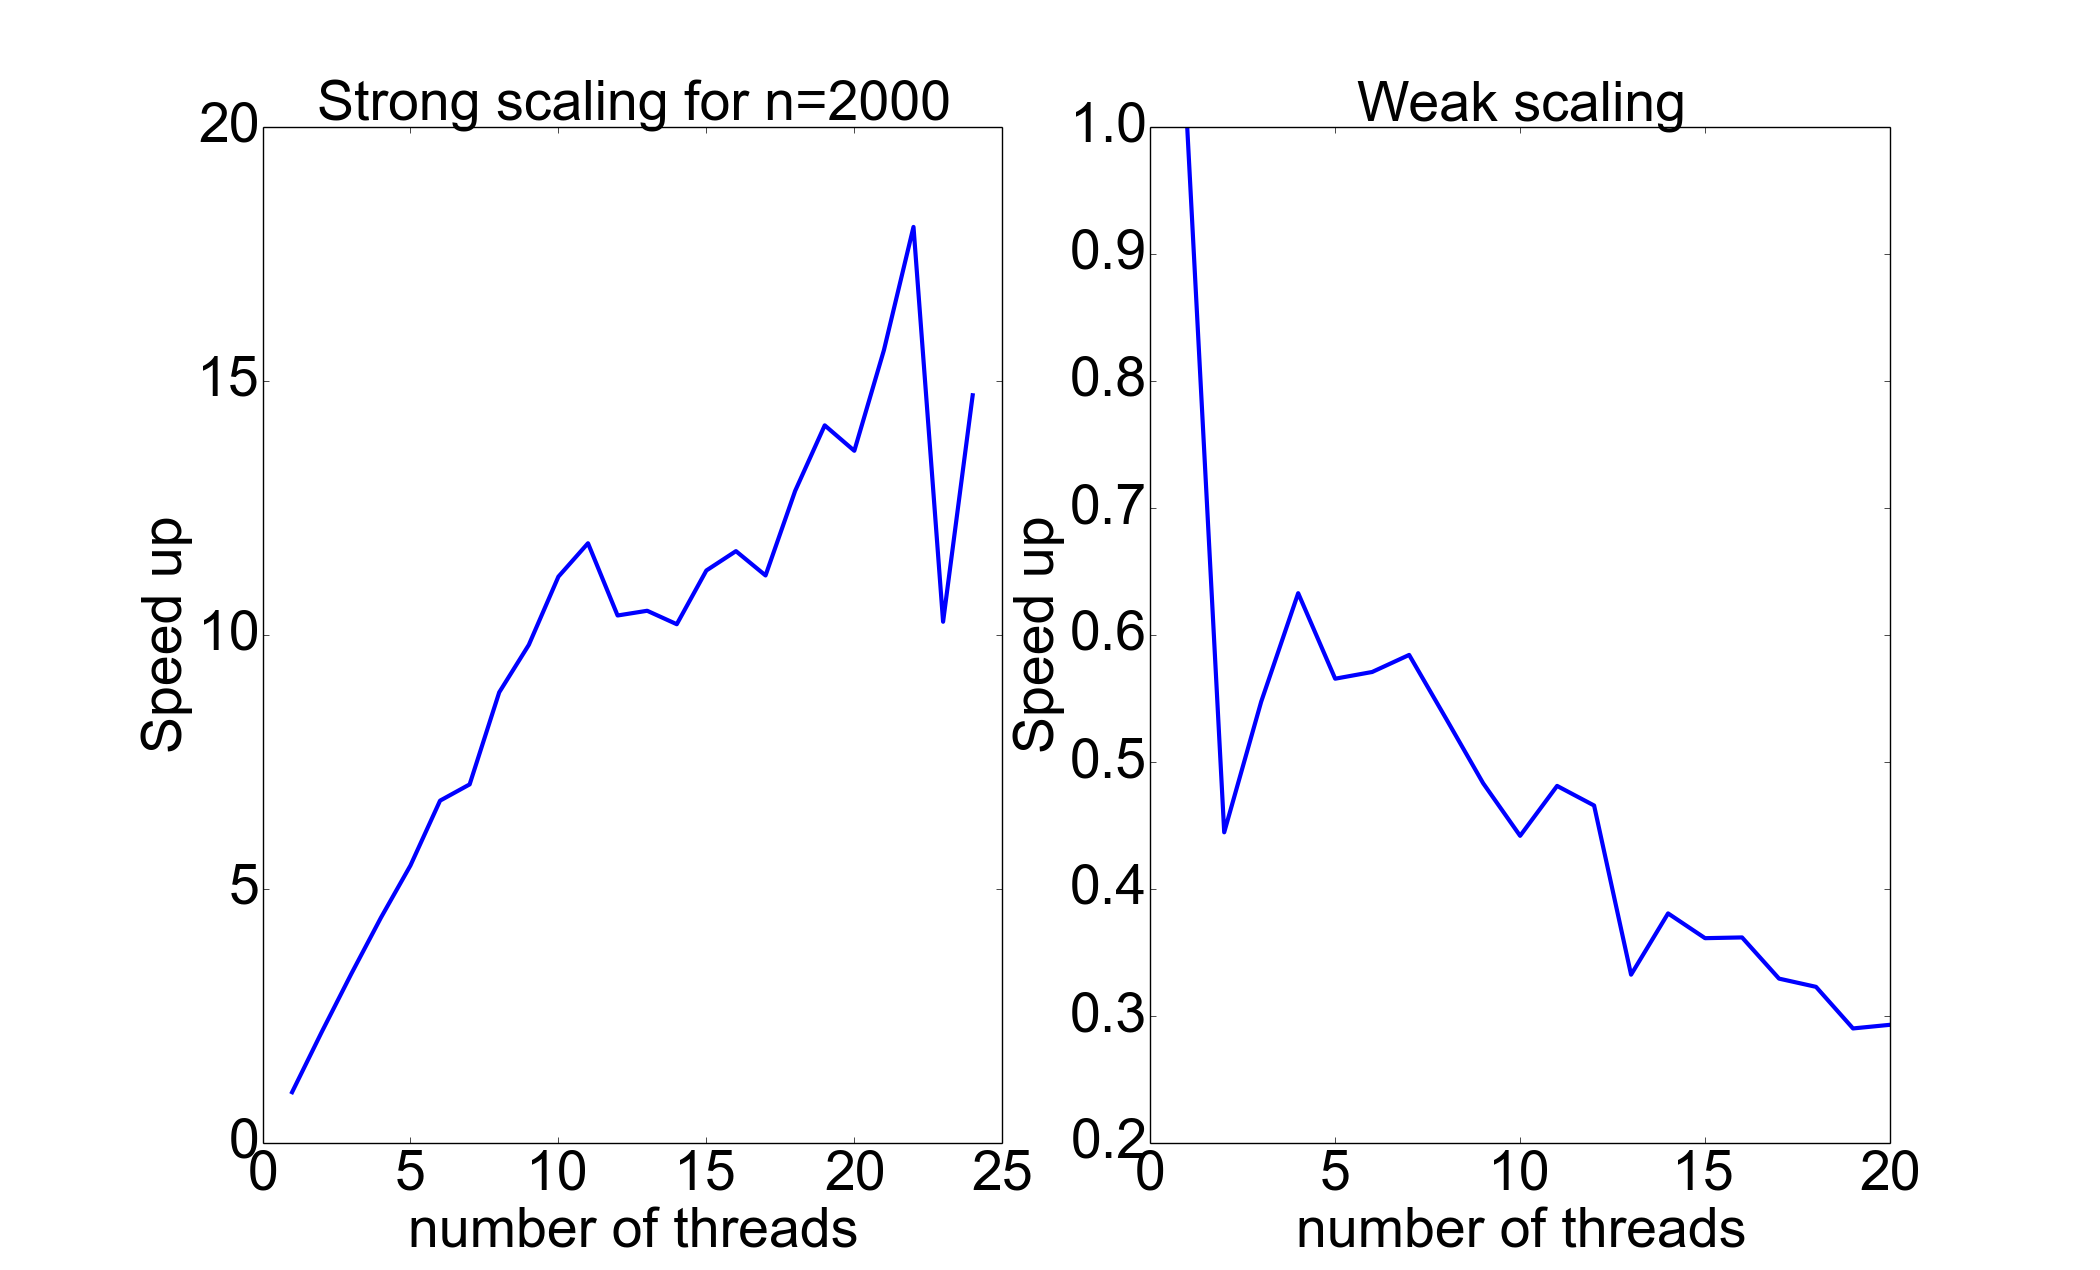
\includegraphics[height=0.4\textwidth, width=\textwidth]{scaling.png}
\end{figure}


\subsection{Weak Scaling}
In weak scaling, you need to increase both the number of processors and the amount of jobs such that each processor has the same amount of jobs. In this problem, the time complexity is O($n^3 \log n$) and we let each processor has approximately O($2000^3\log(2000)$) amount of work. The results are summarized in the right figure of Figure~\ref{scaling}. As can be seen from the right figure of Figure~\ref{scaling}, the speedup is actually decreasing when you increase the amount of work and the number of processors. This could due to the overheading and synchronization when the number of processors is large.

\end{document}
